\documentclass[titlepage,a4paper]{article}

\usepackage{a4wide}
\usepackage[colorlinks=true,linkcolor=black,urlcolor=blue,bookmarksopen=true]{hyperref}
\usepackage{bookmark}
\usepackage{fancyhdr}
\usepackage[spanish]{babel}
\usepackage[utf8]{inputenc}
\usepackage[T1]{fontenc}
\usepackage{graphicx}
\usepackage{float}
\usepackage{listings}
\usepackage{xcolor}

																	% VARIABLES 

\newcommand{\FirstName}{Carlos E.}
\newcommand{\LastName}{Castillo}
\newcommand{\StudentID}{108535}
\newcommand{\StudentEmail}{ccastillo@fi.uba.ar}
% \newcommand{\ProjectName}{Trabajo Práctico n — NombreTP}
\newcommand{\ProjectName}{TDA 3 — Hash}

\pagestyle{fancy}
\fancyhf{}
\fancyhead[L]{TP - \FirstName \LastName}
\fancyhead[R]{Algoritmos y Programación II - FIUBA}
\renewcommand{\headrulewidth}{0.4pt}
\fancyfoot[C]{\thepage}
\renewcommand{\footrulewidth}{0.4pt}

\definecolor{codegreen}{rgb}{0,0.6,0}
\definecolor{codegray}{rgb}{0.5,0.5,0.5}
\definecolor{codepurple}{rgb}{0.58,0,0.82}
\definecolor{backcolour}{rgb}{0.95,0.95,0.92}

\lstdefinestyle{mystyle}{
    backgroundcolor=\color{backcolour},   
    commentstyle=\color{codegreen},
    keywordstyle=\color{magenta},
    numberstyle=\tiny\color{codegray},
    stringstyle=\color{codepurple},
    basicstyle=\ttfamily\footnotesize,
    breaklines=true,                 
    captionpos=b,                    
    keepspaces=true,                 
    numbers=left,                    
    numbersep=5pt,                  
    tabsize=4
}

\lstset{style=mystyle}

\begin{document}
\begin{titlepage}
	\hfill
\includegraphics[width=6cm]{logofiuba.jpg}
    \centering
    \vfill
    \Huge \textbf{\ProjectName}
    \vskip2cm
    \Large [7541/9515] Algoritmos y Programación II\\
    Segundo cuatrimestre de 2021 
    \vfill
    \begin{tabular}{ | l | l | }
      \hline
      Alumno: & \LastName, \FirstName \\ \hline
      Número de padrón: & \StudentID \\ \hline
      Email: & \StudentEmail \\ \hline
  	\end{tabular}
    \vfill
    \vfill
\end{titlepage}

\tableofcontents
\newpage

																 % INTRODUCCION

\section{Introducción}\label{sec:intro}

Muchos lenguajes de programación permiten al usuario extender los tipos de datos
nativos del lenguaje con para facilitar la implementación de características y
funcionalidades más complejas. De esta forma, el programador tiene la capacidad
de combinar diferentes primitivas del lenguaje y así generar nuevos tipos
compuestos para crear interfaces abstractas que faciliten el manejo y
organización de la información mediante diferentes estructuras de datos.

El objetivo de este trabajo práctico es implementar una de las estructuras de
datos más utilizadas, la tabla de hash. 

																		% TEORIA

\section{Teoría}\label{sec:teoria}

\subsection{Tabla de Hash}

El concepto de tabla de hash se deriva de la estructura de datos conocida como
diccionario, una colección de pares clave-valor, en la que cada elemento está
asociado con una clave única con la que es identificado una vez es almacenado en
el diccionario. De esta forma para acceder a los elementos contenidos en el
diccionario se utiliza la misma clave con la que se insertó. Esta estructura de
datos y sus derivados son utilizados principalmente por su capacidad de acceder
rápidamente a la información y evitar la duplicidad de entradas.

\begin{figure}[H]
\centering
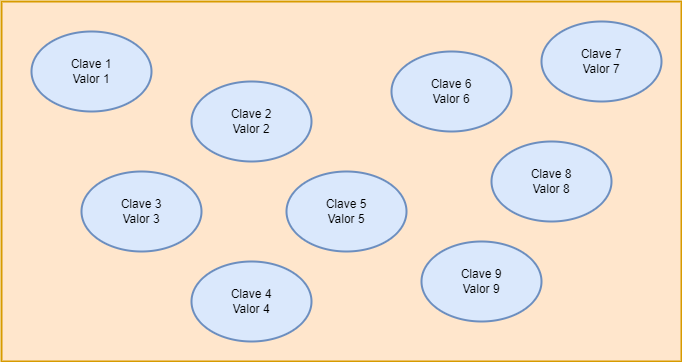
\includegraphics[width=0.8\textwidth]{img/1_diccionario.png}
\caption{\label{fig:seq01}Estructura de Datos Diccionario.}
\end{figure}

En particular una tabla de hash implementa un arreglo asociativo en el que la
ubicación de cada elemento agregado es calculada a traves de una función de
hash, la cual genera un índice dentro del arreglo a partir de la clave
indicada.  Así para insertar, acceder o quitar un elemento almacenado en la
tabla, se toma la clave provista, se encuentra su índice a través de la función
de hash y finalmente se accede a esa posición dentro de la tabla. 

Sin embargo, a medida se van agregando elementos a la tabla, se va aumentando
la probabilidad de que para dos claves distintas se genere un mismo indice de
hash. Cuando esto sucede se dice que hay una ''colisión''. Existen muchas
alternativas para resolver estas colisiones, la mayoría de las cuales implican
cambiar ligeramente la estructura de la tabla o requieren de algún tipo de
reorganización de la información ya almacenada. Las variantes de tablas de hash
más comunes para lidiar con colisiones son la tabla de ''hash abierto'' y tabla
de ''hash cerrado''. 

													 \subsection{Hash Abierto}

Una tabla de hash abierto consiste en una tabla de hash capaz de hacer
encadenamiento o ''chaining'' a los elementos con un mismo indice de hash. Para
esto se suele implementar una estructura de datos secundaria en la que se
almacenarán los elementos que colisionen, generalmente listas enlazadas. De
esta forma la tabla de hash en sí solamente contiene referencias a las
diferentes listas en las que se guardan los elementos. Cada indice de hash
apunta más bien a cada una de estas listas y en caso de colisión, dos pares
clave-valor con el mismo indice de hash van a ser almacenados en la misma
posición en la tabla de hash y encadenados al final de la lista en esa
posición.

\begin{figure}[H]
\centering
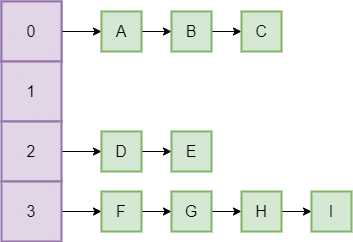
\includegraphics[width=0.5\textwidth]{img/2_hash_abierto.png}
\caption{\label{fig:seq02}Hash Abierto con Listas Enlazadas.}
\end{figure}

Sin embargo uno de los puntos negativos de utilizar este tipo de hash es que
si se van insertando varios elementos con el mismo indice de hash, las listas
enlazadas van a ir aumentando su longitud, haciendo que el tiempo de acceso a
los elementos se tienda a ser $O(n)$ en vez de conservarse como $O(1)$ como es
característico de las estructuras de datos diccionarios. Para evitar esto se
suele hacer una operación conocida como ''rehash'' cuando la cantidad de
elementos en una tabla de hash sobrepasa cierto umbral. Esta operación consiste
en incrementar el número de listas en la tabla y reinsertar nuevamente los
elementos almacenados, ya que al si el indice producido por la función de hash
depende de la cantidad de listas disponibles, al incrementar dicha cantidad,
los indices de elementos previamente almacenados deberán ser reasignados en
base a la nueva cantidad de listas disponibles.

													% DETALLES DE IMPLEMENTACION

				 \section{Detalles de implementación}\label{sec:implementacion}

\begin{lstlisting}[language=C]
struct hash {
	casilla_t** casillas;
	size_t cantidad_casillas;
	size_t cantidad_elementos;
	hash_destruir_dato_t destruir_elemento;
};
\end{lstlisting}

											\subsection{Inserción de elementos}

Se proveen dos funciones para insertar elementos. La primera de estas,
\lstinline{lista_insertar} se encarga de insertar un elemento al final de la
lista y \lstinline{lista_insertar_en_posicion} se encarga de insertar un
elemento en la posición especificada por el usuario. Para esta última función,
en el caso de que el usuario quisiera agregar un elemento en una posición que
no existe en la lista, el elemento se agregará al final de la misma.

Para insertar un elemento en una lista compuesta por nodos enlazados, es
necesario cambiar las referencias de los nodos que anteceden y suceden a la
posición en la que se quiere ubicar el nuevo elemento. Esta operación tiene
varios casos particulares, y para cada uno de estos casos existe una solución
específica:

\begin{itemize}
  \item \textbf{Insertar en una lista vacía:} En este caso la implementación de lista cuenta con dos referencias al primer y último nodo de la lista. Al insertar el primer elemento de una lista vacía, se deben apuntar ambos nodos al mismo elemento.
  \item \textbf{Insertar al inicio de la lista:} Para insertar en esta posición, nuevamente se saca provecho de la existencia de la referencia a un nodo inicial de la lista. Al agregar un elemento en la primera posición primero se establece que el nodo siguiente al nodo que va a ser insertado, es decir, el segundo nodo, va a ser el nodo que actualmente está al inicio de la lista. Luego se cambia referencia la referencia al primer nodo de la lista de tal modo que el nodo que contiene al elemento agregado sea el nuevo primer nodo de la lista. 
  \item \textbf{Insertar al final de la lista:} La operación de insertar en esta posición puede ser vista como la inversa de la operación anterior. Esta vez se utiliza la referencia al elemento que actualmente está al final de la lista, se establece que el elemento siguiente a este último va a ser el nuevo nodo insertado, y finalmente se cambiar la referencia del último nodo de la lista hacia el nuevo nodo.
  \item \textbf{Insertar en cualquier posicion:} Para insertar en cualquier posición de la lista se debe hacer un cambio de referencias similar al de los casos anteriores. Primero se tiene que ubicar el nodo que actualmente se encuentra en la posición anterior a la deseada. Se copia la referencia de este nodo a su nodo siguiente (el nodo que está en la posición deseada) de tal forma que el nuevo nodo a insertar apunte hacia este nodo, y finalmente se hace que el nodo que anterior a la posición deseada tome como nuevo siguiente el nodo que se está insertando.
\end{itemize}

Por último se aumenta la cantidad de elementos en la lista y se retorna el puntero a la lista nuevamente.

Cada destacar que la función \lstinline{lista_insertar} fue implementada de tal manera que esta fuera solamente una manera auxiliar de llamar a la función \lstinline{lista_insertar_en_posicion} especificando la última posición de la lista.

Para la operación de apilado en una pila, se utiliza la misma funcionalidad de inserción que para la lista pero especificando el tope de la pila (posición final) como la única posición de insertado. Por otra parte, para la operación de encolado en una cola, se utiliza esta misma función, nuevamente especificando la posición final de la cola como única posición de insertado posible.


										 \subsection{Eliminación de elementos}

La operación de quitar elementos de la lista tiene una implementación bastante similar a la operación de insertado. También se proveen dos funciones para quitar elementos tanto del final de la lista con la función \lstinline{lista_quitar}, así como también para quitar un elemento de cualquier posición con la función \lstinline{lista_quitar_en_posicion}, la primera de estas funciones siendo un auxiliar de la segunda, en el que se especifica que la posición de eliminado es la última en el caso de la lista.

Al igual que con la inserción de elementos, existen varios casos particulares de eliminación:

\begin{itemize}
  \item \textbf{Quitar del inicio de la lista:} En esta operación se guarda una referencia al nodo a quitar (el primer nodo de la lista) y posteriormente se apunta la referencia de la lista hacia el nuevo primer nodo (que anteriormente era el segundo). Finalmente se almacena el valor que contiene el nodo para retornarlo y se libera la estructura nodo que se removió de la lista.
  \item \textbf{Quitar del final de la lista:} Para quitar un elemento del final de la lista simplemente se guarda una referencia a ese nodo, luego se apunta la referencia de la lista al nodo final hacia el nodo anterior (que anteriormente era el penúltimo), y finalmente se almacena el valor que contiene el nodo para retornarlo y se libera la estructura nodo que se removió de la lista. Al tener una referencia al final de la lista, no se tiene la necesidad de recorrer toda la lista para encontrar el final, así que el tiempo de inserción en el final de la lista es constante si no se requiere de una operación adicional.
  \item \textbf{Quitar de cualquier posición:} Para quitar un elemento de cualquier posición se realiza una operación similar al insertado en cualquier posición, en la que primero guarda una referencia al nodo que se va a eliminar. Luego se localiza el nodo anterior a la posición que se desea quitar en este caso, se cambia la referencia al siguiente nodo para este nodo, y pasa ser el nodo siguiente al que se va a remover. Finalmente se guarda el valor del nodo a quitar para que pueda ser devuelto y se libera la estructura nodo de la memoria.
\end{itemize}

Para las implementaciones de los TDAs pila y cola también se trabaja con las funciones de lista para la operación de remover elementos. En el caso del desapilado en la pila se especifica la única opción de desapilado posible como la posición del tope de la pila (misma posición del último elemento apilado), y para el caso del tipo de dato cola, se especifica la posición de desencolado como la posición del primer nodo de la cola, es decir siempre el que siempre está al frente.

												 \subsection{Otras operaciones}

Además de las operaciones de insertar y quitar se proveen una serie de getters para cada tipo de dato. En el caso de la lista, el usuario puede acceder al primer y último elemento de la misma sin necesidad de remover el elemento, así como también puede acceder a cualquier elemento en medio de la lista. Para acceder al primer y último nodo se utilizan las funciones \lstinline{lista_primero} y \lstinline{lista_ultimo} que toman provecho de las referencias que tiene la lista hacia el nodo inicial y final para realizar esta operación en tiempo constante. Por otra parte, para acceder a cualquier otro elemento se utiliza la función \lstinline{lista_elemento_en_posicion}, la cual si tiene que hacer un recorrido a traves de la lista hasta que encuentra el elemento buscado o \lstinline{NULL} si no se encuentra.

En el caso del tipo de dato pila solo se provee un getter para acceder al elemento del tope, y para el tipo de dato cola, solamente para acceder al elemento del frente.

Para las tres estructuras de datos existen funciones que se encargan de la construcción y destrucción de las mismas, sin destruir la información que tiene almacenada el usuario. Además, las tres estructuras tienen una función retorna la cantidad de elementos que contienen en el momento y otra función que determina si la estructura está vacía o no.


\end{document}

